% @TODO Change this
\chapter{Contour Tree Construction}
\label{chapter3}

%When the domain of the Reeb Graph is a contractable topological space 
Let us now assemble the pieces needed to introduce Contour Trees and their computation - Morse function and simplical complexes.

The Reeb Graph of a contractable topological space is connected and acyclic. This allows us to define this special case of the Reeb Graph as the Contour Tree. In this dissertation we will limit ourselves to practical spacial data analysis where data that is regularly sampled from two or three dimensional Euclidean space. Examples for this are medical imaging [], X-ray crystallography [], terrain mapping data [] and other. 

% @TODO Add Fig
The resolution of any sampling process is limited and if we are to leverage the machinery we have introduced so far we must assume that there is an underlying continuous function present in the space. Our only option in this case is to construct an approximation of this function based on the values we have sampled. This is usually done by constructing a simplicial complex where the data points are the vertices and we add higher dimensional simplicies to completely fill the space between them (see fig[]). The resulting data structure we will call a simplical mesh. The values of the approximation function on the simplicies are obtained via linear interpolation between the verticies of each simplex. 

As long as the original values we have sampled are unique we can show that the resulting linear interpolation function is a Morse function and that the critical values are critical points are the vertices of the mesh. This is one of the key properties that enables efficient computation of the contour tree. We will discuss how to deal with non unique values in the coming sections.

\section{Algorithms for Computing Contour Trees}
In this section we will present the state of the art in current algorithm for contour tree construction. They are based on the work of []. 

Explain more algoirthms.

%\section{Input Data Format}

%% @TODO Add example and citation for irregular domains
%In order to simplify out implementation without much loss in generality we will assume that the input data comes in the form of a real valued $n \times m$ matrix or more appropriately in our context grid. The gird represents the values of vertices of a two dimensional simplicial mesh where the vertices are "evenly spaced" measurements. See example []. The algorithms presented here can be extended to a grid of any number of dimensions or even to irregular grids. See []. 

%The underlying simplicial mesh is assumed to be a triangulation of the vertices [] and the values at the edges and faces of the mesh are obtained through piecewise-linear interpolation based solely on the values of the vertices. Our final assumption is that the input values in the grid are unique. This ensures that the interpolated function is Morse and the it's critical points lie in unique vertices.

%If we are only computing the contour tree of the mesh and not bothering with extracting contours and level sets uniqueness of data values allows us to avoid having to compute the interpolation function and to only work with the values at the vertices of the mesh.

\section{Height Trees}

In order to discuss the algorithms for computing contour tree we must first establish some notation and useful properties about height graphs and trees. A height graph is a graph $G = (V, E)$ together with a real valued function $h$ defined on the vertices of $G$. A height tree is unsurprisingly a height graph which is a tree. Contour trees are examples of height trees and in the spirit of the assumptions we have made about our input data in the previous subsection we will assume all vertices have unique heights. In other words $h(u) \ne h(v)$ for all $u ,v \in V(G)$ where $u \ne v$. The function $h$ naturally induces a total ordering on the vertices. From now on we will assume the vertices of $G$ are given in ascending order. That is to say, $V(G) = \{v_1, v_2, ... , v_n\}$ where $h(v_1) < h(v_2) < ... < h(v_n)$. This lets us work with the indices of the vertices without having to compare their heights directly. In this notation $h(v_i) < h(v_j)$ when $i < j$.

%@TODO Remove this if you will not use it.

Introducing the height function allows us to talk about ascending and descending paths. A path in the graph is a sequence of vertices $(u_1, u_2, ... , u_k)$ where $u_i \in V(G)$ for $i \in \{1, 2, ..., k\}$ and $u_iu_{i+1} \in E(G)$ for $i \in \{1, 2, ..., k-1\}$. Furthermore a path in a height graph is ascending whenever $h(u_1) < h(u_2) < ... < h(u_k)$. Conversely if we traverse the path in the opposite direction it would be descending. We will simply call these paths monotone whenever we wish to avoid committing to a specific direction of travel.

When working with height graphs it is useful to extend the definition of a degree of a vertex by taking the height function into account.

\begin{defn} Let $G$ be a height graph and $v$ a vertex of $G$. The up degree of $v$ is defined as the number of neighbours with higher value. It is denoted as $\delta^+(v) = \big|\{ u \in N(v) : h(u) > h(v) \}\big|$.   \end{defn}

The down degree of $v$ is defined analogously as $\delta^-(v) = \big|\{ u \in N(v) : h(u) < h(v) \}\big|$. 

In the context of height trees the definitions of up and down degrees of a vertex allows us distinguish between two types of leaves - lower and upper leaves.

\begin{defn} Let $G$ be a height graph and $v$ a vertex of $G$. If  $\delta^+(v) = 1$ and $\delta^-(v) = 0$ then $v$ is a lower leaf.  \end{defn}

Conversely if $\delta^+(v) = 0$ and $\delta^-(v) = 1$ then $v$ is an upper leaf. We will see in the next chapter how we can use these two types of leaves to construct the contour tree.

\section{Join and Split Trees}

% @TODO Add example
The contour tree can be associated with two other trees. Those are the join and split trees. They each contain one half of the topological information of the contour tree. The join tree contains information for the contours that join together and the split tree holds the information for the contours that split apart. See example []. More formally the join tree of a contour tree summarises the evolution of the connectivity of the sublevel sets of the interpolation function and the split tree of the superlevel sets. The two are symmetric just as in the way sublevel and super level sets are - relative to the direction of travel of the interpolation function.

Every contour tree is associated with a unique pair of join and split trees. The core idea behind the algorithm for computing the contour tree is that the join and split trees can be combined together to produce the contour tree. The core observation that makes this possible is that the join and split trees of the mesh and of the contour tree of the mesh are the same. The algorithm that is proposed in[] leverages those two insights and has two phases. First it constructs the join and split trees of the mesh and then combines them to obtain the contour tree.

Let us now examine how join and split trees are compute. We will describe for the process for the join tree only as it is completely analogous in the split tree case. 

\begin{defn} A join component is a connected component in the sublevel set $f^{-1}(\{h\})$ at some $h \in \mathbb{R}$.  \end{defn}

Let us now formalise the notion of tracking join components and constructing a join tree. Let us work in the general setting where $X$ is any path-connected topological space and $h : X \to \mathbb{R}$ is a function defined on $X$. The claims we make will hold in the special case where $X$ is a simplicial complex. Let us consider all sublevel sets $X_t = h^{-1}((-\infty, t]) = \{x \in X : h(x) \in (-\infty, t] \}$. They form a one parameter family $\{X_t\}_{t \in \mathbb{R}}$ of nested subsets where $X_a \subseteq X_b$ whenever $a \le b$. What the join tree captures is how the connectivity of the sublevel sets changes as the parameter $t$ is increased. 
    
To visualise this process we can contract every join component to a point much like we did in the Reeb graph. The only difference here is that the equivalence relation is defined for all points in a sublevel set $h^{-1}((-\infty, t])$ instead of a level set $h^{-1}(\{t\})$. Because of this change and because join components can only merge the join tree is a tree. Furthermore if $X_m = X$ is the last sublevel set for some $m \in \mathbb{R}$ then all join components merge into one because $X$ is path connected.

* Here is a beautiful example of this. *

% @TODO Add citation
In order to compute the join tree of our input mesh we will perform an upwards sweep on the vertices. We will use the union-find data structure [] to keep track of which join components vertices are in. Initially all vertices will be places in their unique connected component. At the end of the sweep they will all be in the same component. Then we perform an upwards sweep through the vertices and check if the current vertex merges two or more join components. If it does we add an edge between that vertex and the oldest vertex in the join components in merges in the merge tree.


% @TODO Define Join Saddles and Subdivided edges
Not all vertices of the mesh will be in the join tree. Only those which correspond to local maxima and to join saddles. This will pose a problem upon combining the join and split trees. To avoid this problem we can augment the join tree by adding all missing vertices. This is done through edge subdivision []. Let $a \text{ and } b$ be two adjacent vertices in the join tree.  Let $\{v_1, v_2, ..., v_n\}$ be vertices in the mesh that are not in the join tree that are given in ascending order in terms of height.  Suppose that $h(a) < h(v_i) < h(b)$ for all $i \in \{1, 2, ..., n\}$ and the vertices $v_i$ are in the same connected component of $X_b - h^{-1}(\{b\}) = h^{-1}((-\infty, b))$. In order to augment the join tree with the first vertex we subdivide the edge $ab$ and label the new vertex as $v_1$. Next we subdivide $v_1b$ and label the new vertex as $v_2$. We continue to do so and on the $k$th step we subdivide the edge $v_{k-1}b$ and label the new vertex as $v_k$.

Note that the same augmentation can be applied to the contour tree as well.

* Show some pretty pictures join, aug join, split, aug split, contour, aug contour*

The second step of the algorithm is to combine the join and split trees to produce the contour tree. We will in fact be combining the augmented join tree with the augmented split tree to obtain the augmented contour tree. Removing the augmentation of the contour tree is then left as an optional final step.

The first step in merging the two it to identify all leaves of the contour tree and their incident edges. We can recognize them immediately from the join and split trees using the following property.

\begin{defn} Property of leaves from Hamish's dissertation   \end{defn}


% @TODO Define vertex contraction and quote property.
Once we have those we can remove them from the join and split trees via vertex contraction. Another remarkable we have is that after applying vertex contraction the new join and split are of the subgraph of the contour tree induced by all non-leaves. This means that we can obtain the so called 1nd order leaves (vertices of distance 1 from a leaf) from the new join and split trees by the first property and add those to the contour tree. We can repeat this process iteratively by "pruning" until we have no more vertices left in the join and split trees. Upon reaching this state the contour tree is fully computed.

* See example with pretty pictures *

\section{Serial Algorithm}

To summarise what we obtained so far, here is the overall algorithm for computing the contour tree.

\textbf{Step 1.} Read input grid and convert it to a triangulated mesh.

\textbf{Step 2.} Compute the Join and Split Tree of the input mesh.

\textbf{Step 3.} Iteratively prune leaves and adjacent from the Join and Split tree and add them to the Contour Tree until they are empty.

\textbf{Step 4.} Remove augmentation if necessary and output contour tree.

The running time of this algorithm is $O(n\alpha(n))$ where alpha is the inverse Ackerman function. For all practical intents and purpose the running time of this algorithm is linear. It's space complexity is linear as well.

\section{Parallel Algorithm}

* ----- <roadsign> Peter Construction Co. </roadsign> *


In the year 2016 there was a paper [] published that introduced a data parallel implementation of the contour tree algorithm. The algorithm follows the same two phases of first computing join and split trees and them combining them. We will neglect the details in the new data-parallel way of computing join and split trees as they are not as relevant to the dissertation and the problem we are addressing.  


% @TODO Talk about works and shit and parallelism and add lemma ref
The merge phase of the new algorithm has remained large unchanged. The only difference is that leaves are batched and processed in parallel. This is where the bottleneck of the parallel algorithm lies. Imagine a long chain such as in example []. If we do this approach then our parallel algorithm will be no better than a serial one. We are bottlenecked by the structure of the tree. 

On the other hand if we are able to collapse long chains such as that then effectively we obtain a tree with no vertices of degree two. By out lemma [] we have that at least half of it's vertices will be leaves and all leaves can be processed in parallel.

There is a way to collapse chains with a monotone paths. This is a short description of it. There is however no way to collapse non monotone chain. Therefore long chain with many zig zags in them serialize the parallel algorithm. Out main goal will be to explore long zig zag chains such as that one and try to find a way for the algorithm to collapse them and have logarithmic collapse.

* Explain the zig zags better, but don't go into too much detail until the next chapter.*

\section{Contour Tree Simplification}

Contour Trees are summary of the connectivity of the level sets of a Morse function. They are primarily used in scientific visualisation. A central problem in visualisation is simplifying the data that is presented to enable human comprehension. The contour tree of a large enough data set can quickly become an unwieldy beast in it's own right. This is why it is vital to employ techniques that simplify remove parts of the contour tree that correspond to less "significant" topological features.

One such technique is Branch Decomposition. It was first introduced in \cite{ct-branch-decomp}. It involved decomposing the contour tree into a set of disjoint monotone paths which cover all edges of the tree. This is called branch decomposition and the trivial one is where we take every vertex to be a separate path. A more complex one is shown in this example. Furthermore a branch decomposition is hierarchical when there is exactly one branch that connects two leaves and every other branch connects a leaf to an interior node.

The branches in this scheme represent pair of critical points and form the basis for topological simplification that can be applied. We apply a simplification by removing a branch that does not disconnect the tree. This produces a hierarchy of cancellations like in example []. We define the persistence of a branch to be the bigger of the difference between it's end points and the persistence of it's children. Branches of high persistence reflect more prominent features in the tree. We apply the simplification by removing branches with low persistence that do not disconnect the tree.

\begin{figure}%
    \centering
    \subfloat[Contour Tree.]{{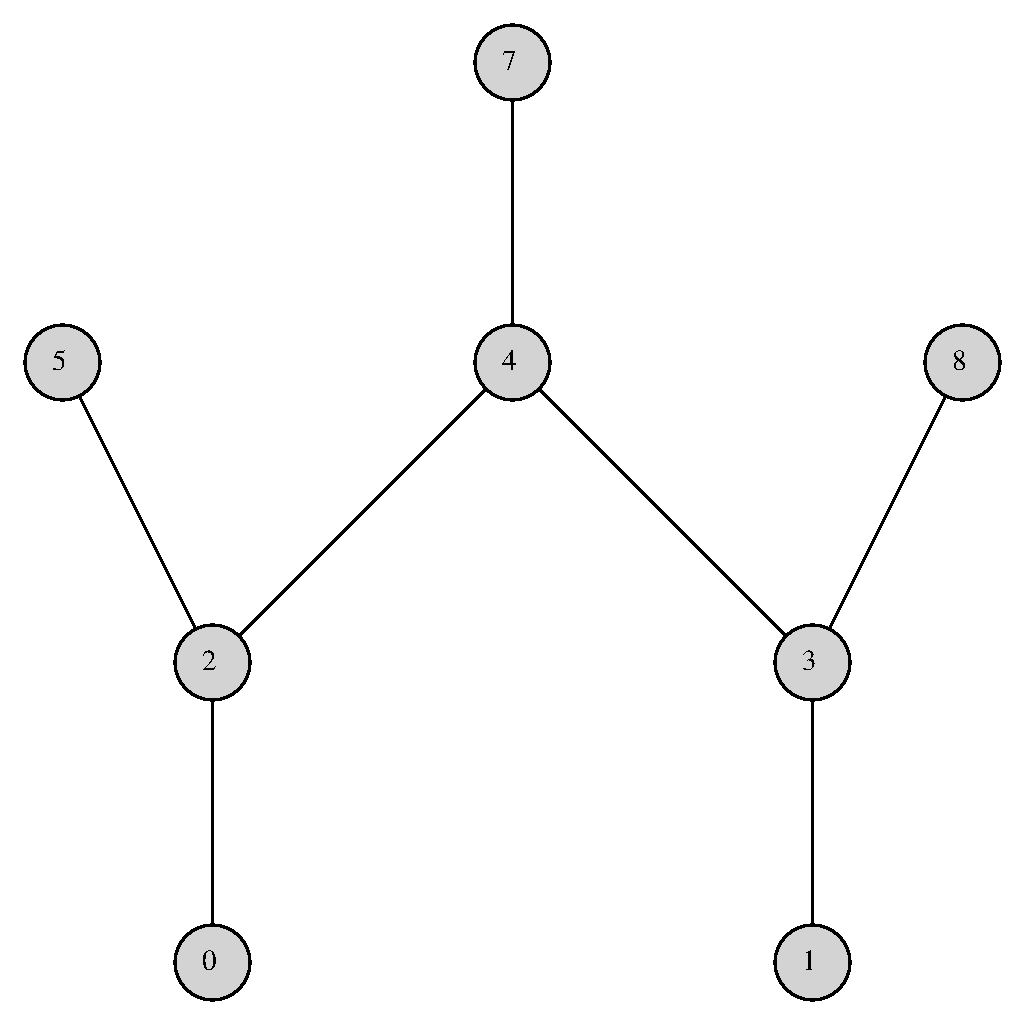
\includegraphics[scale=0.4]{./images/w3x3.eps}}}%
    \qquad
    \subfloat[Branch Decomposition.]{{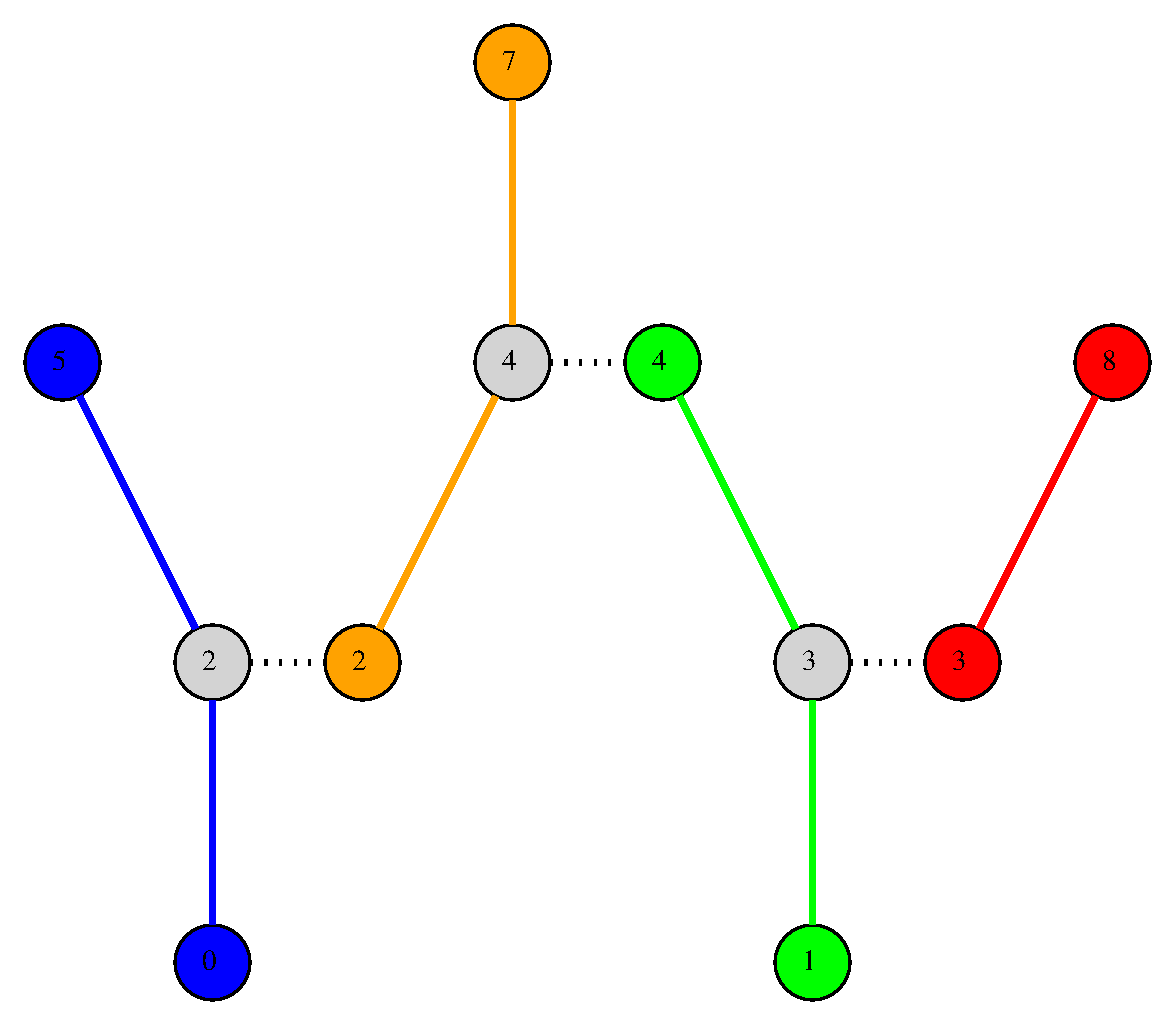
\includegraphics[scale=0.4 ]{./images/branch-decomposition-W3x3.eps}}}%
    \caption{Branch Decomposition of a Contour tree.}%
    \label{fig:example}%
\end{figure}

%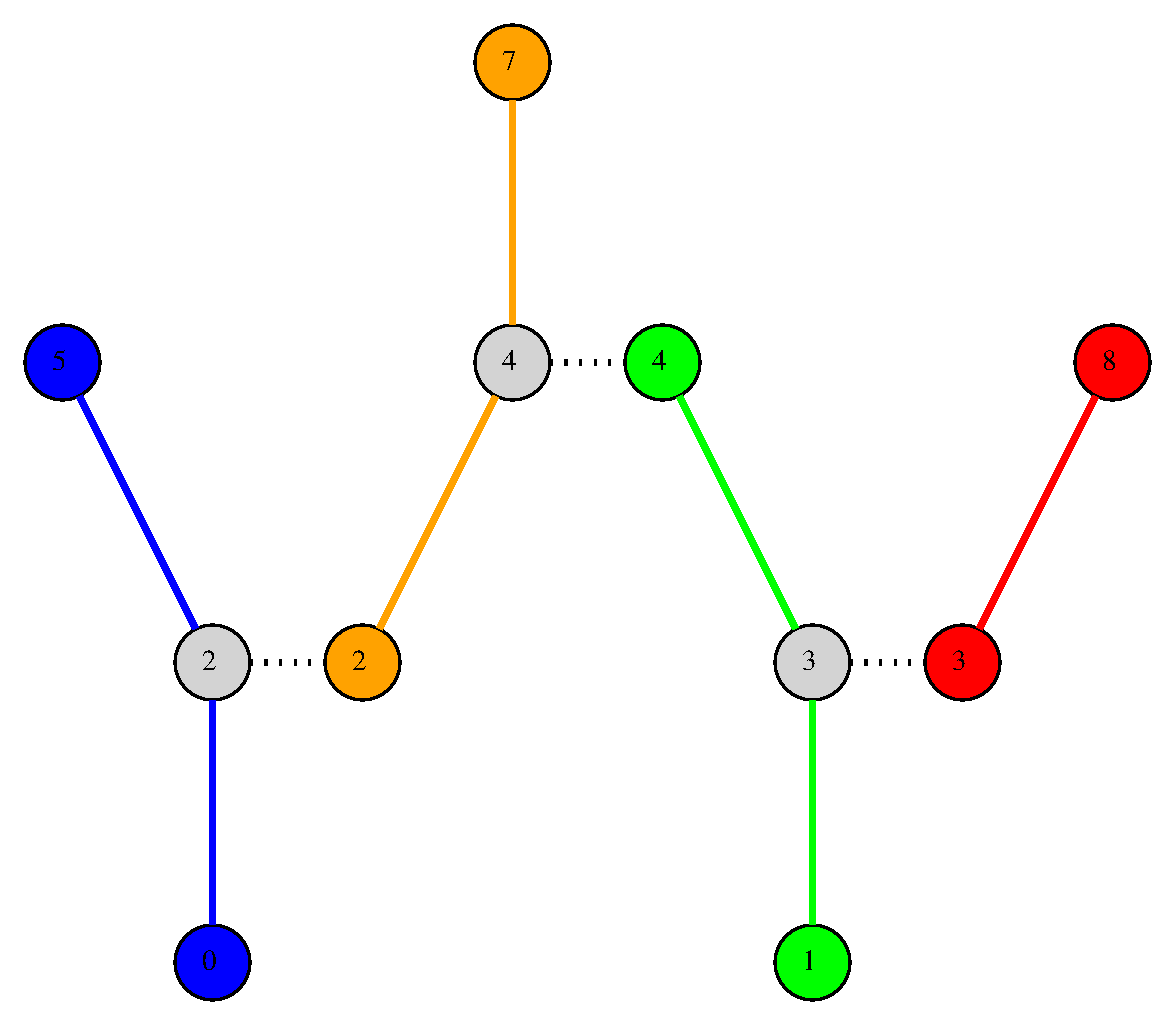
\includegraphics[center, scale=0.5 ]{./images/branch-decomposition-W3x3.eps}
%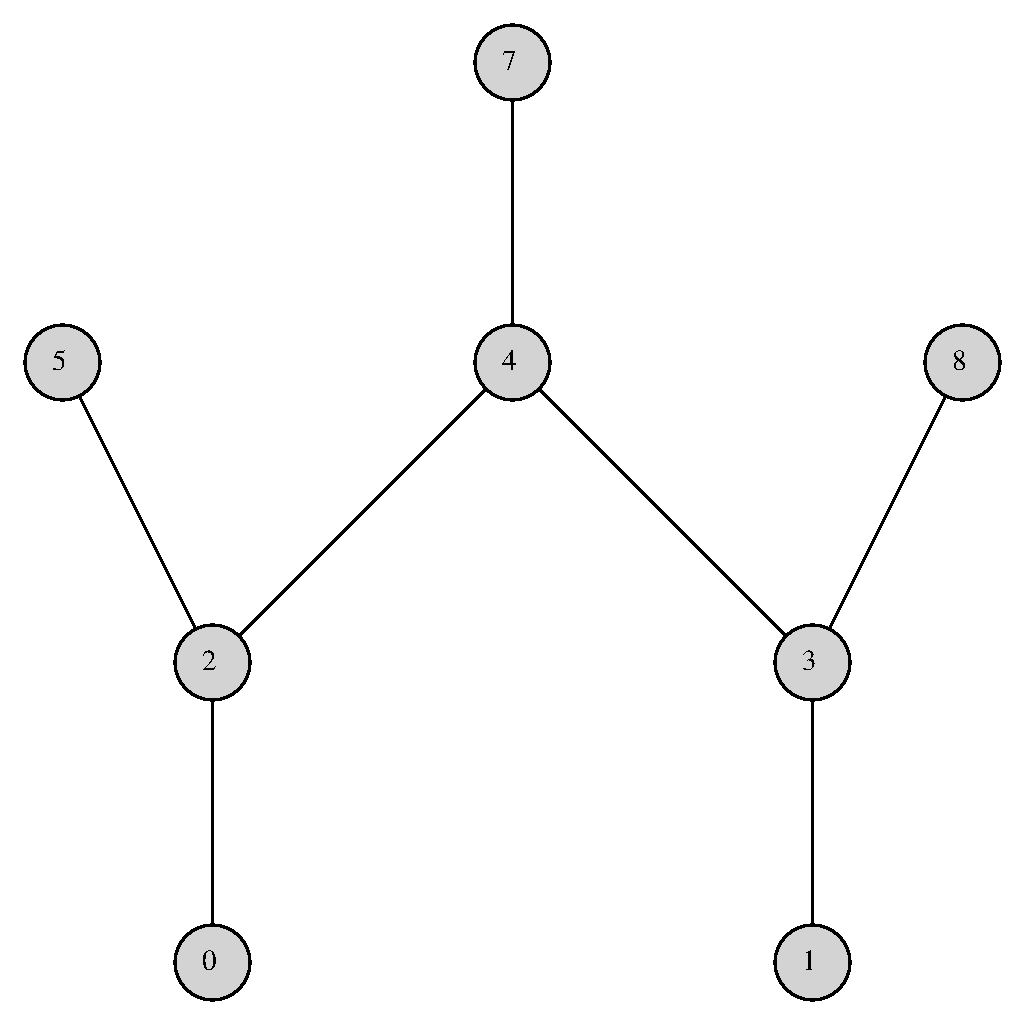
\includegraphics[center, scale=0.5]{./images/w3x3.eps}


% @TODO Todo talk about how this is used to remove noise and artifacts in data.

% @TODO Remove Stay Tuned
The paper \cite{ct-branch-decomp} cites that the persistence defined in that way is similar to persistence first defined in \cite{persistence-original}. In Chapter N of this dissertation we will demonstrate that this claim is either incorrect of misleading. Stay tuned folks.



%First we have to triangulate the mesh.

%Then the mesh is a height graph.

%And the contour tree is a height tree.

%Now define the join and split trees.

%Say they are equal for the mesh and the CT

%Compute the join/split tree of the mesh.

%Now combine them using the combination algorithm.

%There are many algorithms for computing the contour tree. But the Great Khan of all algorithms is the ONE. And then there's the parallel one!
